\chapter[Referêncial bibliográfico]{Referencial bibliográfico}

\section{Classificação de documentos}
\subsection{Técnicas de pré-processamento}
\subsection{Representações de textos}
\subsection{Técnicas de ML}
\subsection{Deep Learning}
%\subsection{Redes Neurais}
%\subsection{Redes Neurais Recorrentes}
%\subsection{Redes Neurais Convolucionais}
\subsection{Métodos de avaliação}

\section{Sistema jurídico brasileiro}

A estrutura do sistema jurídico brasileiro é estabelecido pela Constituição Federal de 1988. Ela prevê quais são os órgãos que compõe o poder judiciário, as competências que eles possuem, onde estão localizados, o tamanho dos representantes das instâncias superiores e como se faz a investidura ao cargo \cite{BRASIL1988}. Além da constituição, para um estudo mais completo, são necessárias as leis federais número 8.457, que estabelece a primeira instância da justiça militar \cite{BRASIL1992} e a número 12.665, a qual define as turmas recursais para segunda instância de juizados especiais \cite{BRASIL2012}.

Para ter um entendimento completo sobre as peças jurídicas e suas origens, é preciso ter conhecimento sobre como está organizado os órgãos do judiciário, pois são através deles que a população vivencia um processo \cite{JUNIOR2012}.

\begin{figure}[h]
	\centering
    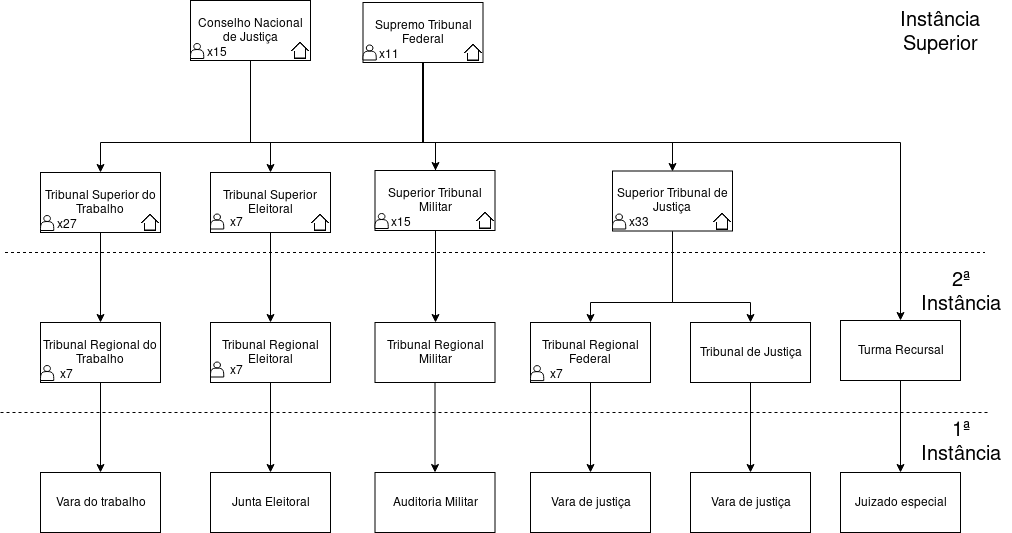
\includegraphics[keepaspectratio=true,scale=0.4]{figuras/sistemaJudiciario}
	\caption[Sistema judiciário]{Organização do sistema jurídico brasileiro. Fonte: elaboração própria}
	\label{fig:sistemaJudiciario}
\end{figure}

Para organizar melhor o trabalho do sistema judiciário, separou-se a justiça comum em algumas áreas para lidar com temas específicos: os assuntos trabalhistas, os eleitorais e uma especialização para lidar com as leis militares \cite{JUNIOR2012}. 

\subsection{Instância superior - Tribunais Superiores}

Como apresentado na Figura \ref{fig:sistemaJudiciario}, são tribunais superiores Supremo Tribunal Federal (STF), Supremo Tribunal de Justiça (STJ), Tribunal Superior Eleitoral (TSE), Tribunal Superior do Trabalho (TST) e Superior Tribunal Militar (STM) \cite{BRASIL1988}.

O STF e o STJ não se encaixam em nenhuma das justiças comum ou especializadas. Pois cabe ao STF a responsabilidade de julgar, em recurso extraordinário, processos que tratam da infração a Constituição e ao STJ julgar, em recurso especial, a não obediência ou ilegitimidade das Leis Federais \cite{BRASIL1988}. Eles não são chamados de terceira instância devido ao princípio da dupla jurisdição. A correta denominação é instância superior, pois em recursos extraordinários, julgam as teses jurídicas e não os fatos do processo \cite{JUNIOR2012}.

Os tribunais TST, TSE e STM compõe também a instância superior, mas estes julgam apenas os recursos de sua área de especialização na justiça \cite{BRASIL1988}.

Todos possuem sua sede na capital do Brasil, e o número mínimo de representantes está estabelecido diretamente na Constituição. Na Figura \ref{fig:sistemaJudiciario}, são representados estes valores para cada um deles. Estes tribunais também possuem a competência para estabelecer o número de servidores nas instâncias inferiores \cite{BRASIL1988}.

\subsection{2ª instância - Tribunais}

Além dos tribunais de segunda instância da justiça especial: o Tribunal Regional Eleitoral, o Tribunal da Justiça do Trabalho e o Tribunal da Justiça Militar, tem-se os tribunais que compõe a justiça comum o Tribunal Regional Federal e os estaduais Tribunal de Justiça \cite{BRASIL1988}. Além destes, há também as turmas recursais que representam a segunda instância para os juizados especiais \cite{BRASIL2012}.

Nestes tribunais, julga-se os recursos ordinários, as provas, as evidências, diferentemente dos tribunais de instância superior \cite{JUNIOR2012}.

\subsection{1ª instância}

Para se entender a organização da justiça de primeira instância, é preciso definir como estão estruturadas a separação da jurisdição dos tribunais.

Cada estado e o Distrito Federal, divide-se em comarcas (ou foros), no qual cada um destes possuem uma ou mais varas especializadas  para as justiças comum e do trabalho \cite{JUNIOR2012}. Para a justiça militar, o território nacional está separado em circunscrições, que cada uma possue sua Auditoria Militar \cite{BRASIL1992}. Já para a justiça eleitoral, existem juntas eleitorais que subdividem os estados e o Distrito Federal em zonas distintas \cite{BRASIL1988}.

A seguir são apresentadas as definições:

\begin{description}
	\item \textbf{Circunscrição} é uma divisão geográfica administrativa para restringir a atuação de um tribunal \cite[p. 71]{GUIMARAES2012}.
	\item \textbf{Comarca} é uma circunscrição sob jurisdição de juízes, na qual o território esta subdividido \cite[p. 75]{GUIMARAES2012}.
    \item \textbf{Vara} é uma repartição judiciária com seu domínio a cargo de um juiz \cite[p. 259]{GUIMARAES2012}.
\end{description}


\section{Código Processual Civil}

O Código Processual Civil (CPC) é um conjunto de leis que definem como devem ser estruturados os processos civis. Ele é o meio pelo qual o juiz concretiza as leis, considerando os interesses entre as partes envolvidas.

Um processo civil possui duas categorias de procedimentos adotados o comum e especial. Neste trabalho tratar-se-á apenas do comum. A seguir, será apresentado para o entendimento das peças jurídicas avaliadas pelo STF, suas características em meio a um processo civil.

\begin{figure}[h]
	\centering
    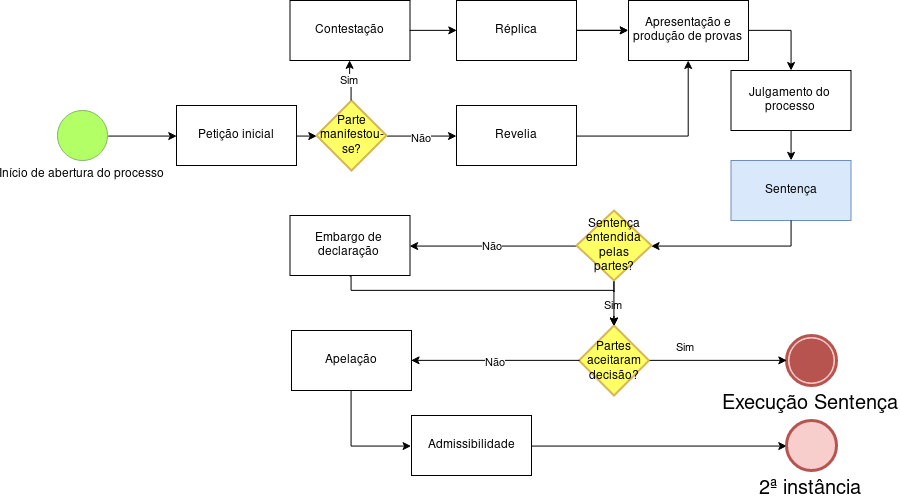
\includegraphics[keepaspectratio=true,scale=0.4]{figuras/processoPrimeira}
	\caption[Processo judiciário - 1ª Instância]{Processo judiciário - 1ª Instância. Fonte: elaboração própria}
	\label{fig:processoPrimeira}
\end{figure}

\subsection{1ª instância}

Um processo civil dar-se início por meio de uma peça chama de petição inicial. Através desta, a parte faz seus pedidos ao juiz e identifica quem é a outra parte, que por sua vez, possui o direito de se manifestar ou não \cite{BRASIL2015}. Chama-se esta fase de postulatória \cite{GONCALVES2016}.

A etapa seguinte é a ordinatória, caracterizada pelo direito de réplica. Depois disso, inicia-se a fase instrutória caracterizada pela produção de provas \cite{GONCALVES2016}.

A etapa decisória tem o ato da sentença \cite{GONCALVES2016}. Deste, é gerada a peça que descreve a decisão tomada pelo juiz mediante os fatos apresentados pelas partes. Uma sentença é inalterável, apenas clarificável pelo pedido de embargo de declaração \cite{BRASIL2015}.

Após a sentença, as partes tem o direito garantido pelo duplo grau de jurisdição de realizar uma apelação. O processo será enviado a um órgão segunda instância caso esteja em conformidade com a lei \cite{GONCALVES2016}.

O artigo 489 do CPC define que existe em todas as sentenças três elementos fundamentais:

\begin{citacao}
I - o relatório, que conterá os nomes das partes, a identificação do caso, com a suma do pedido e da contestação, e o registro das principais ocorrências havidas no andamento do processo;

II - os fundamentos, em que o juiz analisará as questões de fato e de direito;

III - o dispositivo, em que o juiz resolverá as questões principais que as partes lhe submeterem. \cite{BRASIL2015}
\end{citacao}

\subsection{2ª Instância}



\subsection{Instância superior - Superior Tribunal Federal}